\documentclass[14pt]{article}
\usepackage[utf8]{inputenc}
\usepackage[T2A]{fontenc}
\usepackage[uzbek]{babel} 
\usepackage{amsmath, amssymb}
\usepackage{geometry}
\usepackage{graphicx}
\usepackage{xcolor}
\usepackage{hyperref}
\usepackage{tasks}
\usepackage{tcolorbox}
\tcbuselibrary{skins, breakable, theorems}
\usepackage{fancyhdr}
\usepackage{lastpage}
\usepackage{enumitem}
\usepackage{paracol}
\usepackage{ifthen}
\usepackage{needspace}

% Tangens va kotangens komandalari
\newcommand{\tg}{\.operatorname{tg}}
\newcommand{\ctg}{\operatorname{ctg}}

% Geometriya sozlamalari
\geometry{a4paper, left=10mm, right=10mm, top=20mm, bottom=20mm, headheight=15pt}

% Ranglar palitrasi
\definecolor{primary}{RGB}{52, 152, 219}
\definecolor{secondary}{RGB}{46, 204, 113}
\definecolor{accent}{RGB}{155, 89, 182}
\definecolor{lightbg}{RGB}{248, 249, 250}
\definecolor{taskborder}{RGB}{230, 230, 230}
\definecolor{optionbg}{RGB}{240, 242, 245}

% Sahifa foni
\pagecolor{lightbg}

% Giperssilka sozlamalari
\hypersetup{
    colorlinks=true,
    linkcolor=primary,
    urlcolor=primary,
}

% Kolontitullar
\pagestyle{fancy}
\fancyhf{}
\fancyhead[L]{\textcolor{primary}{\textbf{MathCore | MOCK Test-8}}}
\fancyhead[R]{\textcolor{secondary}{Abdunazarov M.X.}}
\fancyfoot[L]{\href{https://t.me/Math_Core_Dtm_MS_Att}{\textcolor{primary}{MathCore}}}
\fancyfoot[R]{\href{https://t.me/Abd_mardon}{\textcolor{secondary}{@Abd\_mardon}}}
\fancyfoot[C]{\textcolor{gray}{\thepage/\pageref{LastPage}}}
\renewcommand{\headrulewidth}{0.5pt}
\renewcommand{\headrule}{\hbox to\headwidth{\color{primary}\leaders\hrule height \headrulewidth\hfill}}
\renewcommand{\footrulewidth}{0.5pt}
\renewcommand{\footrule}{\hbox to\headwidth{\color{secondary}\leaders\hrule height \footrulewidth\hfill}}

% Savol kartochkasi stili
\newtcolorbox{questionbox}[2][]{
    enhanced,
    breakable,
    colback=white,
    colframe=primary,
    coltitle=white,
    fonttitle=\bfseries\large,
    title={Masala \hfill \textcolor{white}{#2}},
    attach boxed title to top left={xshift=5mm, yshift=-2mm},
    boxed title style={size=small, colback=primary, sharp corners},
    sharp corners,
    boxrule=0.5pt,
    left=5mm,
    right=5mm,
    top=5mm,
    bottom=5mm,
    drop fuzzy shadow,
    #1
}

% Javob variantlari stili
\newlist{options}{enumerate}{1}
\setlist[options]{
    label=\textbf{\Alph*)},
    leftmargin=*,
    itemsep=2pt,
    topsep=5pt,
    before={\vspace{2mm}\begin{tcolorbox}[
        colback=optionbg,
        colframe=white,
        sharp corners,
        boxrule=0pt,
        left=2mm,
        right=2mm,
        top=2mm,
        bottom=2mm,
    ]},
    after={\end{tcolorbox}\vspace{2mm}},
}

% Rasmlar uchun komanda
\newcommand{\questionimage}[2][0.5\linewidth]{%
    \begin{center}
        \includegraphics[width=#1]{#2}
    \end{center}
}

\begin{document}

% Titul sahifasi
\begin{center}
    {\Huge \textbf{\textcolor{primary}{MOCK Test-8}}} \\[5mm]
    {\large \textcolor{secondary}{Abdunazarov M.X.}} \\[10mm]
    
\includegraphics[width=0.2\textwidth]{logo.png} \\[5mm]
    \textcolor{gray}{\small Telegram: \href{https://t.me/Math_Core_Dtm_MS_Att}{@Math\_Core\_Dtm\_MS\_Att}}
\end{center}

\vspace{5mm}

% Masala 1
\begin{questionbox}{1}
    Agar \(f(x) = \max\{2;\; x^2 - 1\}\) bo'lsa, \(f(f(0))\) qiymatini toping.
    \begin{options}
        \item 2
        \item 4
        \item 3
        \item 1
    \end{options}
\end{questionbox}

% Masala 2
\begin{questionbox}{2}
    Hisoblang: \(\frac{1}{2} + 1+ \frac{3}{2} + \frac{5}{2} + 3 + ... +\frac{23}{2} + 12\).
    \begin{options}
        \item 40
        \item 56
        \item 78
        \item 150
    \end{options}
\end{questionbox}

% Masala 3
\begin{questionbox}{3}
    \(A, B, C, D, E\) — musbat butun sonlar bo'lib, \(\text{EKUB}(A, B, C) = 4\) va \(\text{EKUB}(C, D, E) = 5\). \(A + B + C + D + E\) yig'indisining eng kichik bo'lishi mumkin bo'lgan qiymatini toping.
    \begin{options}
        \item 22
        \item 38
        \item 36
        \item 47
    \end{options}
\end{questionbox}

% Masala 4
\begin{questionbox}{4}
    \(x^{1803} + 5x^{1802} + 2x^2 + 10x + 7\) ko'phadni \(x + 5\) ga bo'lgandagi qoldiqni toping.
    \begin{options}
        \item 4
        \item 5
        \item 6
        \item 7
    \end{options}
\end{questionbox}

% Masala 5
\begin{questionbox}{5}
    Agar \(a < 0 < b < c\) bo'lsa, \(\frac{|a-b| - |a| - c}{|b-a| - |a-c|}\) ifodaning qiymatini toping.
    \begin{options}
        \item 1
        \item \(-1\)
        \item \(\frac{a}{c}\)
        \item \(-\frac{a}{c}\)
    \end{options}
\end{questionbox}

% Masala 6
\begin{questionbox}{6}
    Agar \(a^2 + \frac{1}{a^2} = 6\) bo'lsa, \(a^3 + \frac{1}{a^3}\) ifodaning qiymatini toping.
    \begin{options}
        \item \(16\sqrt{2}\)
        \item \(10\sqrt{2}\)
        \item \(8\sqrt{2}\)
        \item \(2\sqrt{2}\)
    \end{options}
\end{questionbox}

% Masala 7
\begin{questionbox}{7}
    \((2x-1)^2 (x-2)^4 (x+3)^6 (x+4)^8 \le 0\) tengsizlik nechta butun yechimga ega?
    \begin{options}
        \item \(\varnothing\)
        \item 4
        \item 3
        \item cheksiz ko'p
    \end{options}
\end{questionbox}

% Masala 8
\begin{questionbox}{8}
    Agar \(2^{\log_3(x-1)} - 3^{\log_2(3-x)} = 0\) bo'lsa, \(\log_{\sqrt{2}} x\) ni toping.
    \begin{options}
        \item 0
        \item \(\frac{1}{2}\)
        \item 1
        \item 2
    \end{options}
\end{questionbox}

% Masala 9
\begin{questionbox}{9}
    \(\sqrt{x^2 - 6x + 9} + \sqrt[3]{(x-2)^3} \le \sqrt[5]{(x+2)^5}\) tengsizlikni nechta butun son qanoatlantiradi?
    \begin{options}
        \item 9
        \item 7
        \item 8
        \item 6
    \end{options}
\end{questionbox}

% Masala 10
\begin{questionbox}{10}
    \(f(x) = \cos(x+5) + \operatorname{tg}^4(x+1)\) funksiyaning eng kichik musbat davrini toping.
    \begin{options}
        \item \(\frac{\pi}{4}\)
        \item \(\frac{\pi}{2}\)
        \item \(\frac{3\pi}{2}\)
        \item \(2\pi\)
    \end{options}
\end{questionbox}

% Masala 11
\begin{questionbox}{11}
    \(8,\; 16,\; 32,\; 56,\; \dots\) ketma-ketlikda qo'shni hadlarining ayirmasi arifmetik progressiyani tashkil etadi. Ushbu ketma-ketlikning 1688 ga teng bo'lgan hadi raqamini toping.
    \begin{options}
        \item 22
        \item 21
        \item 19
        \item 20
    \end{options}
\end{questionbox}

% Masala 12
\begin{questionbox}{12}
    Chizmada ko'rsatilgan to'g'ri chiziqlardagi nuqtalarni uchlari deb hisoblab, nechta uchburchak hosil qilish mumkin?
    \begin{center}
        
\includegraphics[width=0.5\linewidth]{1.png}
    \end{center}
    \begin{options}
        \item 15
        \item 22
        \item 30
        \item 32
    \end{options}
\end{questionbox}

% Masala 13
\begin{questionbox}{13}
    Firmada 7 nafar erkak va 3 nafar ayol ishlaydi. Tavakkaliga 3 kishi tanlab olindi. Tanlanganlarning barchasi erkak bo'lishi ehtimolligini toping.
    \begin{options}
        \item \(\frac{3}{32}\)
        \item \(\frac{11}{28}\)
        \item \(\frac{7}{24}\)
        \item \(\frac{5}{12}\)
    \end{options}
\end{questionbox}

% Masala 14
\begin{questionbox}{14}
    \(\left( \sqrt{x} - \frac{2}{x} \right)^n\) yoyilmasining ozod hadi 60 ga teng. \(n\) ni toping.
    \begin{options}
        \item 3
        \item 4
        \item 5
        \item 6
    \end{options}
\end{questionbox}

% Masala 15
\begin{questionbox}{15}
    Mergan uchun nishonga urish ehtimolligi 0,8 ga teng. 5 ta o'q uzildi. Dastlabki 3 ta o'q nishonga tekkanligi, keyingi 2 tasi esa tegmaganligi ehtimolligini toping.
    \begin{options}
        \item \(2^{10} \cdot 10^{-6}\)
        \item \(2^{11} \cdot 10^{-5}\)
        \item \(2^{11} \cdot 10^{-6}\)
        \item \(2^{10} \cdot 10^{-5}\)
    \end{options}
\end{questionbox}

% Masala 16
\begin{questionbox}{16}
    \(f(x) = \frac{g(x)+1}{3h(x)-1}\) funksiya uchun \(g(3) = 0,\; h(3) = 2,\; h'(3) = 1,\; g'(3) = 2\) ma'lum bo'lsa, \(f'(3)\) ni toping.
    \begin{options}
        \item \(\frac{5}{19}\)
        \item \(\frac{7}{19}\)
        \item \(\frac{7}{25}\)
        \item \(\frac{6}{25}\)
    \end{options}
\end{questionbox}

% Masala 17
\begin{questionbox}{17}
    Chizmada \(y = x^2 - 8x + m\) funksiya grafigi tasvirlangan. Agar \(|OB| = 3|OA|\) bo'lsa, \(m\) ni toping.
    \begin{center}
       
\includegraphics[width=0.3\linewidth]{2.png}
    \end{center}
    \begin{options}
        \item \(14\)
        \item 12
        \item 10
        \item \(6\)
    \end{options}
\end{questionbox}

% Masala 18
\begin{questionbox}{18}
    Hisoblang: \[\int_9^{10}(x-9)^8 xdx\]
    \begin{options}
        \item \(1\frac{1}{10}\)
        \item \(1\frac{1}{8}\)
        \item \(1\frac{1}{9}\)
        \item \(1\frac{1}{11}\)
    \end{options}
\end{questionbox}

% Masala 19
\begin{questionbox}{19}
    Agar \(f(x+1)+x\cdot f(2)=x^2+3\) bo'lsa, \(f(3)\) ni toping.
    \begin{options}
        \item \(3\)
        \item \(4\)
        \item \(7\)
        \item \(8\)
    \end{options}
\end{questionbox}

% Masala 20
\begin{questionbox}{20}
    Hisoblang: \[\int_0^{3/2}\left( \sqrt{9-x^2} - \sqrt{3}x\right)dx\]
    \begin{options}
        \item \(\frac{\pi}{2}\)
        \item \(\pi\)
        \item \(\frac{3\pi}{2}\)
        \item \(\frac{3\pi}{4}\)
    \end{options}
\end{questionbox}

% Masala 21
\begin{questionbox}{21}
    Keltirilgan ma'lumotlardan foydalanib, bo'yalgan soha yuzini toping.
    \begin{center}
        
\includegraphics[width=0.3\linewidth]{3.png}
    \end{center}
    \begin{options}
        \item 8
        \item 10
        \item 12
        \item 14
    \end{options}
\end{questionbox}

% Masala 22
\begin{questionbox}{22}
    Quyidagi tasdiqlardan qaysilari to'g'ri?
    \begin{enumerate}
        \item Uchburchakka ichki chizilgan doira yuzi \(\frac{\pi}{4}\left(\frac{4S}{a+b+c}\right)^2\) formula bilan ifodalanadi (bunda \(a, b, c\) — uchburchak tomonlari, \(S\) — uning yuzi);
        \item O'xshash shakllar yuzalarining nisbati mos burchaklar sinuslarining kvadratiga teng;
        \item Balandliklari va asos radiuslari teng bo'lgan konus va silindr hajmlarining nisbati 3 ga teng;
        \item Silindr yon sirti yuzi \(2\pi R(R+h)\) formula bilan topiladi;
        \item Har qanday ko'pburchakning (har bir uchidan bittadan olingan) tashqi burchaklari yig'indisi \(360^\circ\) ga teng.
    \end{enumerate}
    \begin{options}
        \item 1,5
        \item 2,3,5
        \item 3,4
        \item 1,2,5
    \end{options}
\end{questionbox}

% Masala 23
\begin{questionbox}{23}
    Trapetsiyada \(DC \parallel EF \parallel AB\), \(DC = 4\), \(AB = 2\sqrt{13}\). \(EF\) kesma uzunligini toping.
    \begin{center}
        \centering
        
\includegraphics[width=0.5\linewidth]{6.png}
    \end{center}
    \begin{options}
        \item \(\sqrt{34}\)
        \item \(4\sqrt{2}\)
        \item \(\sqrt{30}\)
        \item \(2\sqrt{7}\)
    \end{options}
\end{questionbox}

% Masala 24
\begin{questionbox}{24}
    \(ABCD\) va \(CBFE\) — kvadratlar, \(AD = 6\). \(O_1\) va \(O_2\) nuqtalar (kvadratlar markazlari) orasidagi masofani toping.
    \begin{center}
        
\includegraphics[width=0.5\linewidth]{8.png}
    \end{center}
    \begin{options}
        \item \(2\)
        \item \(3\sqrt{3}\)
        \item \(3\)
        \item \(2\sqrt{2}\)
    \end{options}
\end{questionbox}

% Masala 25
\begin{questionbox}{25}
    Chizmada muntazam oltiburchak tasvirlangan. Agar \(S_{KDE} = 3\) bo'lsa, bo'yalgan soha yuzini toping.
    \begin{center}
      
\includegraphics[width=0.3\linewidth]{7.png}
    \end{center}
    \begin{options}
        \item 78
        \item 39
        \item 54
        \item 27
    \end{options}
\end{questionbox}

% Masala 26
\begin{questionbox}{26}
    Uchburchak balandliklari 6, 6 va 15 ga teng. Shu uchburchak yuzini toping.
    \begin{options}
        \item \(90\sqrt{6}\)
        \item \(36\sqrt{15}\)
        \item \(\frac{225}{2\sqrt{6}}\)
        \item \(\frac{270\sqrt{3}}{5}\)
    \end{options}
\end{questionbox}

% Masala 27
\begin{questionbox}{27}
    \((x-a)^2 + (y-12)^2 = 25\) aylanadan \(4x + 3y - 14 = 0\) to'g'ri chiziqqacha bo'lgan eng qisqa masofa 5 ga teng. \(a\) ni toping (\(a > 0\)).
    \begin{options}
        \item 5
        \item 6
        \item 8
        \item 7
    \end{options}
\end{questionbox}

% Masala 28
\begin{questionbox}{28}
    \(ABC\) uchburchak yuzi 12 ga, \(BD = 3\) ga teng. \(x = KC\) ni toping.
    \begin{center}
       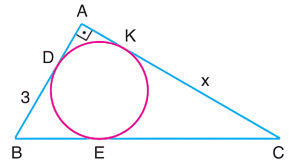
\includegraphics[width=0.5\linewidth]{21.png}
    \end{center}
    \begin{options}
        \item 4
        \item 5
        \item 6
        \item 7
    \end{options}
\end{questionbox}

% Masala 29
\begin{questionbox}{29}
    Teng yonli uchburchakning yon tomoni 20 ga, asosi 24 ga teng. Medianalar kesishish nuqtasidan ichki chizilgan aylana markazigacha bo'lgan masofani toping.
    \begin{options}
        \item 1
        \item \(\frac{1}{3}\)
        \item \(\frac{2}{3}\)
        \item \(\frac{1}{2}\)
    \end{options}
\end{questionbox}

% Masala 30
\begin{questionbox}{30}
    Asos radiusi 5 bo'lgan to'g'ri silindrda (chizma) I holatda suv balandligi \(12\sqrt{3}\) ga teng. Silindr asosi gorizontal tekislik bilan \(30^\circ\) burchak hosil qiladigan qilib egilganda (II holat), suv darajasi \(AD\) tomonidagi \(K\) nuqtaga yetadi. \(AK\) uzunligini toping.
    \begin{center}
      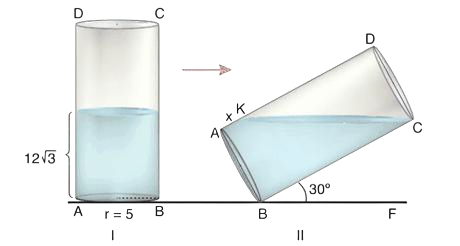
\includegraphics[width=0.5\linewidth]{22.png}
    \end{center}
    \begin{options}
        \item \(4\sqrt{3}\)
        \item \(5\sqrt{3}\)
        \item \(6\sqrt{3}\)
        \item \(7\sqrt{3}\)
    \end{options}
\end{questionbox}

% Masala 31
\begin{questionbox}{31}
    Asos radiusi 2 m va balandligi 4 m bo'lgan to'g'ri konus shaklidagi idishga doimiy tezlikda suv quyilmoqda. Suv chuqurligi \(y\) metr bo'lganda, idishdagi suv hajmi (\(\pi\) m\(^3\) hisobida) \(y\) orqali qanday ifodalanadi:
    \begin{center}
      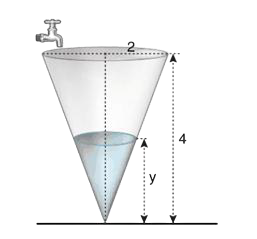
\includegraphics[width=0.5\linewidth]{32.png}
    \end{center}
    \begin{options}
        \item \(\frac{y^3}{3}\)
        \item \(2y^3\)
        \item \(\frac{y^3}{12}\)
        \item \(\frac{y^3}{8}\)
    \end{options}
\end{questionbox}

% Masala 32
\begin{questionbox}{32}
    Muntazam to'rtburchakli prizmaning diagonali \(6\sqrt{3}\) ga teng. Prizmaning balandligi qanday bo'lganda uning hajmi eng katta bo'ladi?
    \begin{options}
        \item \(6\sqrt{2}\)
        \item 6
        \item \(2\sqrt{3}\)
        \item \(2\sqrt{6}\)
    \end{options}
\end{questionbox}

% Masala 33
\begin{questionbox}{33}
    Piramidaning asosi muntazam oltiburchakdan iborat. Piramida balandligi 8 ga, asos tomoni \(4\sqrt{3}\) ga teng. Piramida apofemasini toping.
    \begin{options}
        \item \(8\sqrt{3}\)
        \item 10
        \item \(16\sqrt{3}\)
        \item 12
    \end{options}
\end{questionbox}

% Masala 34
\begin{questionbox}{34}
    Radiusi 6 bo'lgan silindr uning o'qidan 3 masofada o'tuvchi tekislik bilan kesilgan. Hosil bo'lgan kesim yuzi o'q kesimi yuzidan necha marta kichik?
    \begin{options}
        \item \(\sqrt{3}\)
        \item \(\frac{2\sqrt{3}}{3}\)
        \item \(\sqrt{2}\)
        \item \(\frac{3\sqrt{3}}{2}\)
    \end{options}
\end{questionbox}

% Masala 35
\begin{questionbox}{35}
    Konus asosiga tomoni \(6\sqrt{3}\) bo'lgan muntazam uchburchak ichki chizilgan. Konus yasovchisi 10 ga teng. Uning hajmini toping.
    \begin{options}
        \item \(48\pi\)
        \item \(72\pi\)
        \item \(96\pi\)
        \item \(36\pi\)
    \end{options}
\end{questionbox}

\end{document}